\chapter{Background}
\label{sec:Background}

\section{Open MPI}
\label{sec:openmpi}
``The Open MPI Project is an open source Message Passing Interface implementation that is developed and maintained by a consortium of academic, research, and industry partners. Open MPI is therefore able to combine the expertise, technologies, and resources from all across the High Performance Computing community in order to build the best MPI library available. Open MPI offers advantages for system and software vendors, application developers and computer science researchers.\\
Features implemented or in short-term development for Open MPI include:
\begin{itemize}
  \item Full MPI-3 standards conformance
  \item Thread safety and concurrency
  \item Dynamic process spawning
  \item Network and process fault tolerance
  \item Support network heterogeneity
  \item Single library supports all networks
  \item Run-time instrumentation
  \item Many job schedulers supported
  \item Many OS's supported (32 and 64 bit)
  \item Production quality software
  \item High performance on all platforms
  \item Portable and maintainable
  \item Tunable by installers and end-users
  \item Component-based design, documented APIs
  \item Active, responsive mailing list
  \item Open source license based on the BSD license''~\cite{openmpi}
\end{itemize}
    
\subsection{The Architectire of Open MPI}
Open MPI is built based on a component architecture called the Modular Component Architecture (MCA). Component based archtirecture makes large software projects extensible and maintainable~\cite{barrett2005analysis,graham2006open}. It also allows users to build their own costumized components and integrate it into Open MPI. Component based architectures are popular in the high performance computing community~\cite{squyres2003component,bernholdt2006component}.

Open MPI is comprised of three main functional areas (Figure \ref{fig:MCA_framework})~\cite{graham2006open}:

\begin{figure}[h!]
\centering

\includegraphics[scale=0.4]{images/MCA_framework.png}
\caption{MCA, component frameworks, and the components}
\label{fig:MCA_framework}
\end{figure}

\begin{enumerate}
\item \textbf {MCA}\\
  The backbone modular component architecture that provides management services for all other layers.
  
  The MCA is responsible for management of the component frameworks and providing them services they use. For instance, the MCA provides the ability to accept run-time parameters from higher-level abstractions (e.g., mpirun) and pass them down through the component framework to individual components. It also finds components at build-time and invokes their corresponding hooks for configuration, building, and installation.
  
\item \textbf{Component frameworks}\\
  Each major functional area in Open MPI has a corresponding back-end component framework, which manages modules.
  
  Each component framework is a construct that is created for a single, targeted task. For example, \textbf{btl} (Byte Transfer Layer) framework is used to send and receive data on different types of networks, \textbf{allocator} framework is responsible for memory allocation, and \textbf{coll} framework which is dedicated to MPI collective algorithms. A framework uses MCA's services to discover, load, use, and unload components at run time. Each framework has different policies and use case scenarios; some only use one component at a time while others use all available components simultaneously.

\item \textbf {Components}\\
  Self-contained software units that can configure, build, and install themselves. A component is an implementation of a framework's interface. Components are also known as ``plugins''. Each instance of a component is called a ``module''. 

  The Open MPI software has three classes of components: Open MPI (OMPI) components, Open Run Time Environment (ORTE) components, and Open Portable Access Layer (OPAL) components. (Figure \ref{fig:open-mpi-layers})

  Frameworks, components, and modules can be either dynamic or static. This means, they can be available as plugins or they can be compiled statically into libraries.
\end{enumerate}

\begin{figure}[h!]
\centering
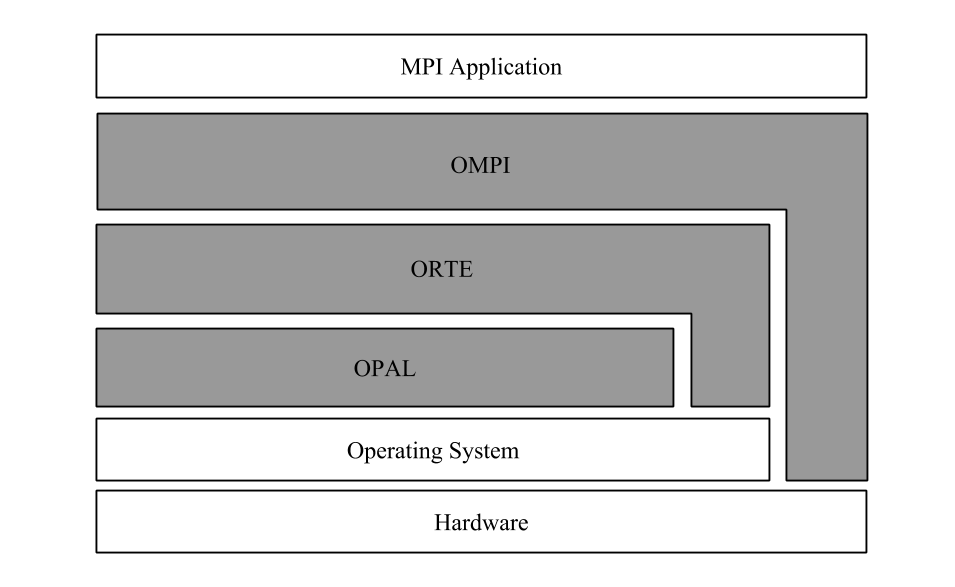
\includegraphics[scale=0.5]{images/open-mpi-layers.png}
\caption{Open MPI layers}
\label{fig:open-mpi-layers}
\end{figure}


\section{Open Runtime Environment (ORTE)}
\label{sec:orte}
Developing software environments for high performance computing applications in heterogenous distributed systems poses a significant challenge. The runtime environment (RTE) must be capable of supporting heterogeneous operations, efficiently scaling from one to large numbers of processors, and providing effective strategies for dealing with fault scenarios that are expected as our systems continue to scale~\cite{kronstadt2005peta}.

There has been a number of studies with different approaches to this challenge. Each approach focuses on a particular aspect of the overall problem. For example, LAM/MPI emphasis was on ease of portability and performance~\cite{squyres2004component}. LA-MPI focused on data fault tolerance~\cite{aulwes2004architecture}, and HARNESS FT-MPI focused on system fault tolerance~\cite{fagg2002harness}.

The Open Run Time Environment (ORTE) was developed as a part of the Open MPI project to support distributed high performance computing applications operating in a heterogeneous environment. Implementation of the ORTE is based on the Modular Component Architecture (MCA). The main design objectives of the ORTE are ease of use, resilient operations, scalability, and extensibility. Interprocess communication, resource discovery and allocation, and process launch across different platforms in a transparet manner are main features of the ORTE.\cite{castain2005open,Castain2008153,castain2008open}.

``The major roles of the runtime are:
\begin{itemize}
\item \textbf{Launch:} Launch the MPI application’s processes. This role is shared between the implementation runtime and the parallel machine scheduling / launching mechanism.
\item \textbf{Connect:} Help the MPI library establish the necessary connections between the processes. Depending on the network used, hardware or configuration specific issues, the connection information (also known as the business card, or the URI of
a process) may not be known before the MPI processes are launched. It is then necessary to distribute this information through an out-of-band messaging system. In most MPI implementations, this role is dedicated to the runtime.
\item \textbf{Control:} Control the MPI processes: ensure that in case of a crash the entire environment is gracefully cleaned; depending on the operating system and implementation, forward signals to the MPI processes; ensure that completion codes
are returned to the user command: mpirun.
\item \textbf{IO:} Forward the standard input/output: users usually expect that the information printed on the standard output should appear on the standard output of the command they launched. Because the command they launched does not necessarily run on the same machine as where the print is issued in an MPI application, it is necessary to ensure the transmission of this information.''~\cite{bosilca2011scalability}
\end{itemize}

\section{High Performance ParalleX (HPX)}
\label{sec:hpx}
ParalleX is a new computation model that attempts to address the underlying sources of performance degradation (starvation, latency, overhead, and waiting) and the difficulties of programmer productivity like explicit locality management and scheduling, performance tuning, fragmented memory, and synchronous global barriers to dramatically enhance the broad effectiveness of parallel processing for high end computing.~\cite{4228212}




